\documentclass{article}
\usepackage[paperwidth=33cm,paperheight=9.5cm,margin=0cm]{geometry}
\usepackage[utf8]{inputenc}
\usepackage[T1]{fontenc}
\usepackage{lmodern}
\usepackage{amsmath}
\usepackage{amssymb}
\usepackage{tikz}
\usetikzlibrary{shapes.geometric, positioning, arrows.meta, fit, backgrounds, calc, decorations.markings, shapes.misc}

\pagestyle{empty}

\begin{document}
\centering
\vspace*{\fill}
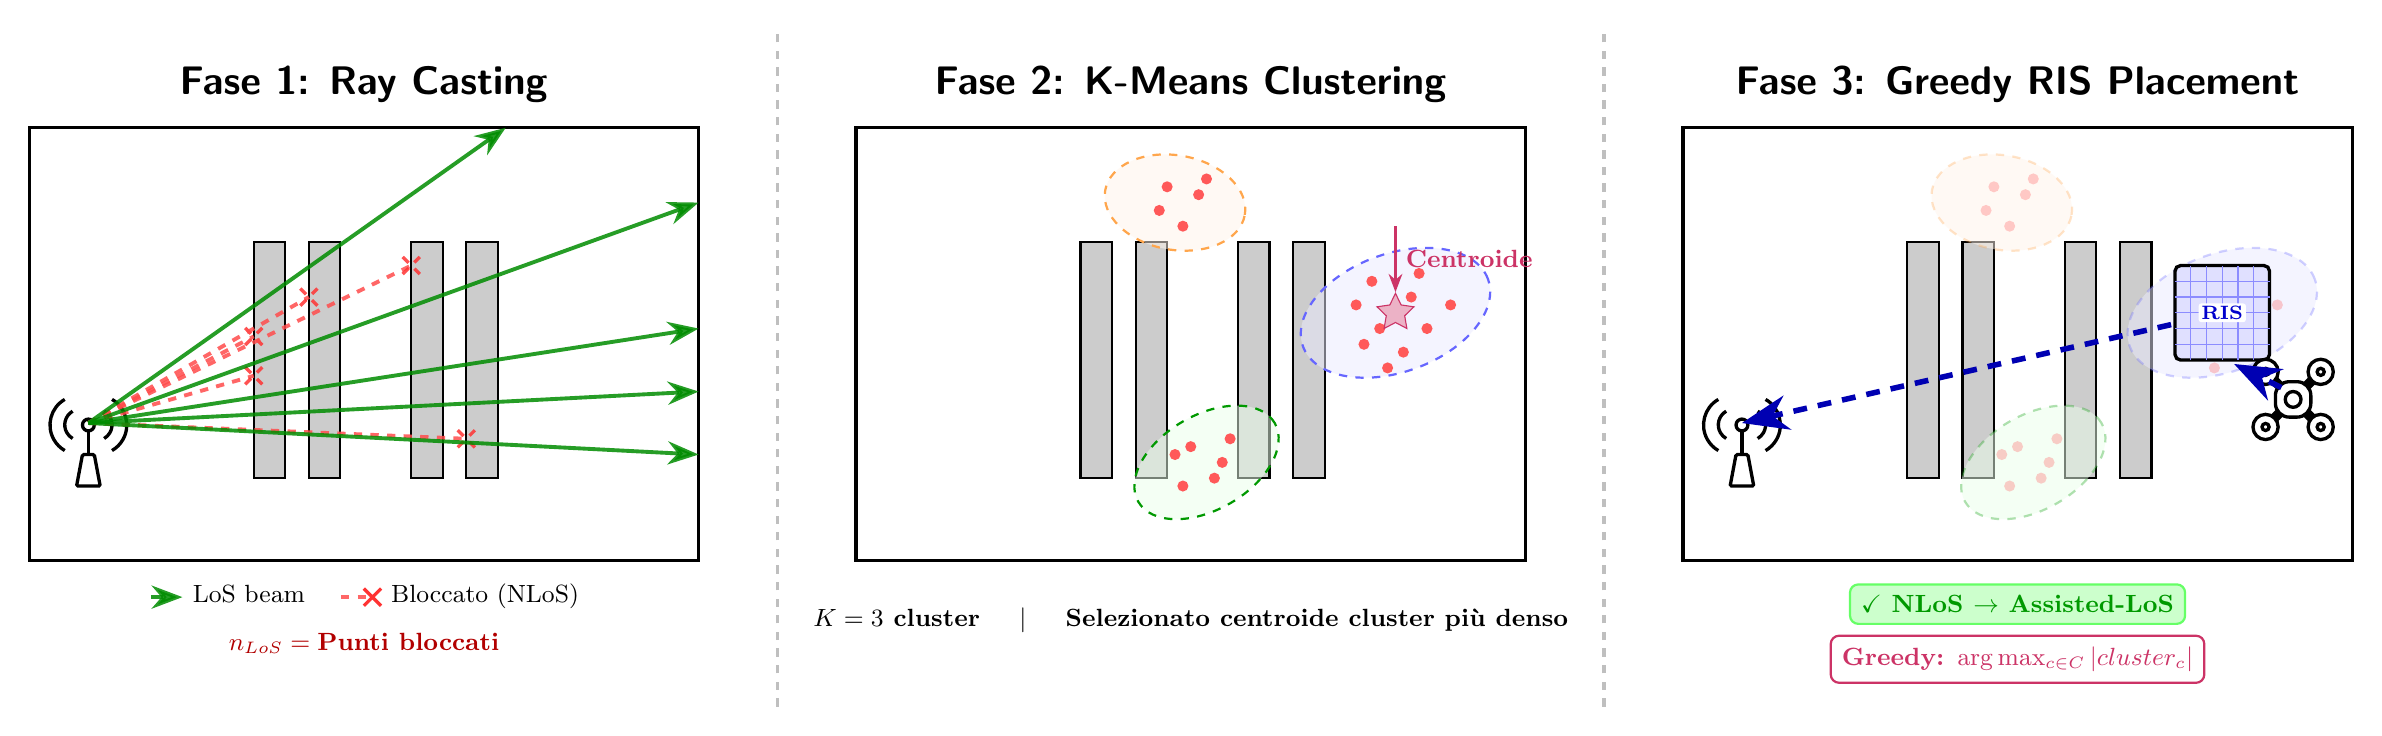
\begin{tikzpicture}[
    font=\sffamily,
    warehouse_walls/.style={
        draw=black, very thick,
        minimum width=8.5cm, minimum height=5.5cm,
        fill=white, inner sep=0pt
    },
    shelf/.style={
        draw=black, fill=gray!40, thick,
        minimum width=0.4cm, minimum height=3cm
    },
    los_beam/.style={
        -{Stealth[scale=1.2]}, green!55!black, line width=1.4pt, opacity=0.85
    },
    nlos_beam/.style={
        -, red!70, line width=1.4pt, dashed, opacity=0.85
    },
    hit_mark/.style={
        cross out, draw=red!80, very thick, inner sep=2.5pt, minimum size=5pt
    },
    nlos_point/.style={
        circle, fill=red!65, minimum size=4pt, inner sep=0pt
    },
    cluster_1/.style={
        ellipse, draw=blue!60, dashed, thick, fill=blue!8, fill opacity=0.5, text opacity=1, rotate=20
    },
    cluster_2/.style={
        ellipse, draw=orange!70, dashed, thick, fill=orange!8, fill opacity=0.5, text opacity=1, rotate=-10
    },
    cluster_3/.style={
        ellipse, draw=green!60!black, dashed, thick, fill=green!8, fill opacity=0.5, text opacity=1, rotate=30
    },
    centroid_mark/.style={
        star, star points=5, star point ratio=2, draw=purple!80, fill=purple!30,
        minimum size=14pt, inner sep=0pt
    },
    glow_circle/.style={
        circle, draw=purple!50, fill=purple!15,
        line width=2pt, minimum size=26pt
    },
    badge_ok/.style={
        rounded corners=3pt, fill=green!20, draw=green!60,
        thick, inner sep=4pt, font=\small\bfseries\color{green!60!black}
    },
    alos_line/.style={
        -{Stealth[scale=1.4]},
        blue!70!black, line width=2pt,
        dashed, dash pattern=on 5pt off 4pt
    }
]

%% ── BS Symbol ──────────────────────────────
\tikzset{bs/.pic={
    \begin{scope}[scale=0.50]
    \draw[very thick, fill=white, rounded corners=0.5pt]
        (-0.3,0)--(0.3,0)--(0.15,0.8)--(-0.15,0.8)--cycle;
    \draw[very thick](0,0.8)--(0,1.4);
    \draw[very thick, fill=white](0,1.55) circle(0.15);
    \draw[very thick](0.4,1.9)  arc(60:-60:0.40);
    \draw[very thick](0.6,2.2)  arc(60:-60:0.75);
    \draw[very thick](-0.4,1.9) arc(120:240:0.40);
    \draw[very thick](-0.6,2.2) arc(120:240:0.75);
    \end{scope}
}}

%% ── Drone Symbol ───────────────────────────
\tikzset{drone/.pic={
    \begin{scope}[scale=0.50]
    \draw[line width=3.5pt](-0.7,-0.7)--(0.7,0.7);
    \draw[line width=3.5pt](-0.7,0.7)--(0.7,-0.7);
    \draw[very thick, fill=white, rounded corners=5pt]
        (-0.45,-0.45) rectangle (0.45,0.45);
    \draw[very thick, fill=white](0,0) circle(0.20);
    \foreach \x/\y in {-0.7/-0.7, 0.7/0.7, -0.7/0.7, 0.7/-0.7}{
        \draw[very thick, fill=white](\x,\y) circle(0.32);
        \draw[very thick, fill=white](\x,\y) circle(0.09);
    }
    \end{scope}
}}

%% ── RIS Symbol – QUADRATA ─
\tikzset{ris_sq/.pic={
    \begin{scope}
    \draw[very thick, fill=blue!12, rounded corners=2pt]
        (-0.6,-0.6) rectangle (0.6,0.6);
    \foreach \x in {-0.4,-0.2,0.0,0.2,0.4}{
        \draw[blue!45, thin](\x,-0.6)--(\x,0.6);
        \draw[blue!45, thin](-0.6,\x)--(0.6,\x);
    }
    \node[font=\scriptsize\bfseries, text=blue!80!black, fill=white, inner sep=1pt, rounded corners=1pt] at (0,0) {RIS};
    \end{scope}
}}

% ══════════════════════════════════════
%  PANNELLO 1 – Ray Casting
% ══════════════════════════════════════
\begin{scope}[shift={(0,0)}]
    \node[warehouse_walls] (w1) at (0,0) {};
    \node[anchor=south, yshift=5pt] at (w1.north)
        {\textbf{\Large Fase 1: Ray Casting}};
    
    \pic at (-3.5,-1.8) {bs};

    \foreach \x in {-1.2, -0.5, 0.8, 1.5}{
        \node[shelf] at (\x,-0.2) {};
    }

    % Beams
    \coordinate (bs_ant) at (-3.5, -1.0);
    
    \draw[nlos_beam] (bs_ant) -- (-1.4, -0.4) node[hit_mark] {};
    \draw[nlos_beam] (bs_ant) -- (-1.4, 0.1) node[hit_mark] {};
    \draw[nlos_beam] (bs_ant) -- (-0.7, 0.6) node[hit_mark] {};
    \draw[nlos_beam] (bs_ant) -- (0.6, 1.0) node[hit_mark] {};
    \draw[nlos_beam] (bs_ant) -- (1.3, -1.2) node[hit_mark] {};
    
    \draw[los_beam] (bs_ant) -- (4.25, -1.4);
    \draw[los_beam] (bs_ant) -- (4.25, -0.6);
    \draw[los_beam] (bs_ant) -- (4.25, 0.2);
    \draw[los_beam] (bs_ant) -- (4.25, 1.8);
    \draw[los_beam] (bs_ant) -- (1.8, 2.75);
    
    % Legenda
    \node[font=\small] at (0, -3.2) {
        \tikz[baseline=-0.5ex]{\draw[los_beam] (0,0)--(0.4,0);} LoS beam \quad
        \tikz[baseline=-0.5ex]{\draw[nlos_beam] (0,0)--(0.4,0); \node[hit_mark] at (0.4,0) {};} Bloccato (NLoS)
    };
    
    \node[font=\small\bfseries, text=red!70!black] at (0, -3.8) {$n_{LoS} = \text{Punti bloccati}$};
\end{scope}

% ══════════════════════════════════════
%  PANNELLO 2 – Algoritmo K-Means
% ══════════════════════════════════════
\begin{scope}[shift={(10.5,0)}]
    \node[warehouse_walls] (w2) at (0,0) {};
    \node[anchor=south, yshift=5pt] at (w2.north)
        {\textbf{\Large Fase 2: K-Means Clustering}};

    \foreach \x in {-1.2, -0.5, 0.8, 1.5}{
        \node[shelf] at (\x,-0.2) {};
    }
    
    % Punti NLoS e Clusters
    % Cluster A (Blu) - zona densa a destra
    \node[cluster_1, minimum width=2.5cm, minimum height=1.5cm] at (2.6, 0.4) {};
    \foreach \p in {(2.1,0.5), (2.4, 0.2), (2.3, 0.8), (2.7, -0.1), (2.8, 0.6), (3.0, 0.2), (2.5, -0.3), (2.9, 0.9), (3.3, 0.5), (2.2, 0.0)}{
        \node[nlos_point] at \p {};
    }
    
    % Cluster B (Arancio) - in alto
    \node[cluster_2, minimum width=1.8cm, minimum height=1.2cm] at (-0.2, 1.8) {};
    \foreach \p in {(-0.4, 1.7), (0.1, 1.9), (-0.1, 1.5), (0.2, 2.1), (-0.3, 2.0)}{
        \node[nlos_point] at \p {};
    }
    
    % Cluster C (Verde) - in basso
    \node[cluster_3, minimum width=2.0cm, minimum height=1.2cm] at (0.2, -1.5) {};
    \foreach \p in {(0.0, -1.3), (0.3, -1.7), (0.5, -1.2), (-0.1, -1.8), (0.4, -1.5), (-0.2, -1.4)}{
        \node[nlos_point] at \p {};
    }
    
    % Centroide
    \node[centroid_mark] (centroid) at (2.6, 0.4) {};
    
    % Annotazioni
    \draw[-Stealth, thick, purple!80] (2.6, 1.5) -- (centroid.north) node[midway, right, font=\small\bfseries\color{purple!80}] {Centroide};
    
    \node[font=\small\bfseries, text=black] at (0, -3.5) {$K=3$ cluster \quad $|\quad$ Selezionato centroide cluster pi\`{u} denso};
    
\end{scope}

% ══════════════════════════════════════
%  PANNELLO 3 – Algoritmo Greedy
% ══════════════════════════════════════
\begin{scope}[shift={(21,0)}]
    \node[warehouse_walls] (w3) at (0,0) {};
    \node[anchor=south, yshift=5pt] at (w3.north)
        {\textbf{\Large Fase 3: Greedy RIS Placement}};

    \pic at (-3.5,-1.8) {bs};

    \foreach \x in {-1.2, -0.5, 0.8, 1.5}{
        \node[shelf] at (\x,-0.2) {};
    }
    
    % Background clusters sbiaditi
    \begin{scope}[opacity=0.3]
        \node[cluster_1, minimum width=2.5cm, minimum height=1.5cm] at (2.6, 0.4) {};
        \foreach \p in {(2.1,0.5), (2.4, 0.2), (2.3, 0.8), (2.7, -0.1), (2.8, 0.6), (3.0, 0.2), (2.5, -0.3), (2.9, 0.9), (3.3, 0.5), (2.2, 0.0)}{
            \node[nlos_point] at \p {};
        }
        \node[cluster_2, minimum width=1.8cm, minimum height=1.2cm] at (-0.2, 1.8) {};
        \foreach \p in {(-0.4, 1.7), (0.1, 1.9), (-0.1, 1.5), (0.2, 2.1), (-0.3, 2.0)}{
            \node[nlos_point] at \p {};
        }
        \node[cluster_3, minimum width=2.0cm, minimum height=1.2cm] at (0.2, -1.5) {};
        \foreach \p in {(0.0, -1.3), (0.3, -1.7), (0.5, -1.2), (-0.1, -1.8), (0.4, -1.5), (-0.2, -1.4)}{
            \node[nlos_point] at \p {};
        }
    \end{scope}

    % Glow del centroide
    \node[glow_circle] at (2.6, 0.4) {};
    
    % RIS piazzata esattamente sul centroide
    \coordinate (ris_pos) at (2.6, 0.4);
    \pic at (ris_pos) {ris_sq};

    % Drone nella zona buia
    \pic at (3.5, -0.7) {drone};
    
    % Path Drone -> RIS -> BS
    \draw[alos_line] (3.35, -0.55) -- (2.75, -0.25);
    \draw[alos_line] (1.95, 0.25) -- (-3.5, -1.0);
    
    % Badge
    \node[badge_ok] at (0, -3.3) {\checkmark\ NLoS $\rightarrow$ Assisted-LoS};

    % Label math greedy
    \node[draw=purple!80, fill=white, thick, rounded corners=3pt, inner sep=4pt, font=\small\bfseries\color{purple!80}] at (0, -4.0) {Greedy: $\arg\max_{c \in C} |cluster_c|$};

\end{scope}

% ══════════════════════════════════════
%  DIVISORI
% ══════════════════════════════════════
\draw[dashed, gray!50, very thick] (5.25, -4.6) -- (5.25, 4.0);
\draw[dashed, gray!50, very thick] (15.75, -4.6) -- (15.75, 4.0);

\end{tikzpicture}
\vspace*{\fill}
\end{document}
